\section{Reflective spaces}
$X$ banach, $X^*=\mathcal L(X,\mathbb R)$ banach too
\paragraph{Notation} $L\in X^*, \ x\in X$
$$Lx=L(x)=\langle L,x\rangle_X$$

\subsubsection{(def) bidual of $X$}
the bidual of $X$ is the dual of $X^*$
$$X^{**}=(X^*)^*=\mathcal L(X^*,\mathbb R)$$
What are the relations between $X$ and $X^{**}$
Fixing a point (a vector) in the starting space $X$m then we can construct an element $\Lambda_x\in X^{**}$ as $$\Lambda_x(L)=Lx$$
More formally, $\Lambda_x=\tau(x)$
$$\tau:X\xrightarrow[\ \ \ \ \ \ \ \ \ \ ]{}X^{**}$$
$$\ _{X^{**}}\langle\Lambda_x,L\rangle_{X^*}=\ _{x^{*}}\langle L,x\rangle_{X}$$
$\tau$ is called "canonical map" or "evaluation map".
\subsubsection{prop}
$\forall x\in X, \Lambda_x\in X^{**}$ and 
$$\Vert \Lambda_x\Vert _{**}=\Vert x\Vert $$
(in other words, $\tau$ is an isometry between $X$ and $X^{**}$).
\begin{proof}\ 
    \begin{enumerate}
        \item $\Lambda_x$ is linear: $\ _{**}\langle \Lambda_x,L\rangle _*=\ _{X^*}\langle L,x\rangle_X$ so it follows from the linearity of $\langle\cdot,\cdot\rangle$.
        $$\Lambda_x(\alpha L_1+\beta L_2)=\ _{X^*}\langle \alpha L_1+\beta L_2,x\rangle_X=$$
        $$=\alpha \langle L_1,x\rangle +\beta \langle L_2,x\rangle=\alpha \Lambda_xL_1+\beta \Lambda_xL_2$$
        \item $\Lambda_x$ is bounded: implied by "isometry"
        $$\Vert \Lambda_x\Vert_{**}=\sup_{L\neq 0}\frac{|\Lambda_xL|}{\Vert L\Vert_*}=\frac{|Lx|}{\Vert L\Vert _*}$$
        now I can look for a bound from above and a bound from below. If I'm sharp, I will find the exact value of the norm.
        \begin{enumerate}
            \item $$\sup_{L\neq 0}\frac{|Lx|}{\Vert L\Vert_*}\leq \sup_{L\neq 0}\frac{\Vert L\Vert_*\cdot \Vert x\Vert}{\Vert L\Vert_*}=\Vert x\Vert$$
            \item $$\sup_{L\neq 0}\frac{|Lx|}{\Vert L\Vert_*}\geq \frac{|\bar Lx|}{\Vert \bar L \Vert_*}$$
            From Corollary \#1 of Hahn-Banach, if $x\neq 0$, $\exists \tilde L_= \ :\ \tilde L_0x=\Vert x\Vert $ s.t. $\Vert \tilde L_0\Vert =1$
            So we can chose $\bar L=\tilde L_0$
            $$\frac{|\bar Lx|}{\Vert \bar L \Vert_*}=\frac{|\tilde L_0x|}{1}$$
        \end{enumerate}
        
        
    \end{enumerate}
\end{proof}
\subsubsection{(thm)}
$$\tau:X\xrightarrow[\ \ \ \  \ ]{}X^{**}$$
is:
\begin{itemize}
    \item linear, continuous
    \item isometry
    \item injective
    \item $R(\tau)\subset X^{**}$ closed
    \item a continuous embedding
\end{itemize}
\paragraph{Lemma (nice properties of linear isometries)}
Take:
\begin{itemize}
    \item $X,Y$ to be Banach spaces;
    \item $T:X\xrightarrow[\quad\quad]{}Y$ a linear operator s.t. $\Vert Tx\Vert_Y=\Vert x\Vert_X,\quad \forall x\in X$
\end{itemize}
Then:
\begin{itemize}
    \item $T$ is continuous
    \item $T$ is injective
    \item $R(T)\subset Y$ is closed
    \item $T:X\xrightarrow[\quad]{}R(T)$ is an isomorphism
\end{itemize}
\begin{proof}
    To prove the theorem we use the lemma above.
    \begin{enumerate}
        \item     Since $T$ linear $\implies T$ continuous $\iff T$ bounded,\\
    $$\Vert Tx\Vert_Y\leq M\Vert x\Vert_X\quad \forall x$$
    is isometry $\implies \Vert Tx\Vert_Y=\Vert x\Vert$, so we can just choose $M=1$ and prove the inequality.
    \item $x,y\in X$ s.t. $Tx=Ty$, $T(x-y)=0$, $$\Vert x-y\Vert =\Vert T(x-y)\Vert _Y=\Vert 0\Vert_Y=0$$
    $$\implies x=y \text{ (injectivity)}$$
    \item To show that $R(T)$ is closed I have to show that 
    $$\begin{cases}\{y_n\}_n\subset R(T)\\ y_n\to \bar y\in Y\end{cases}\implies \bar y\in R(T)$$
    Use $y_n=Tx_n\implies y_n-y_m=T(x_n-x_m)\implies\Vert y_n-y_m\Vert_Y=\Vert x_n-x_m\Vert_X$\\
    We observe that $\{y_n\}$ is a Cauchy sequence, so (from the line above) $\{x_n\}$ is a Cauchy sequence. Since $X$ is banach, $x_n\to \bar x$ and so $y_n=Tx_n$
    \item Since $T\in \mathcal L(X,R(T))$ and $R(T)$ is closed $\implies $ Banach.
    $T$ is bijective between $X$ and $R(T)$. $\implies T^{-1}$ continuous by a corollary of the open mapping theorem.
    \end{enumerate}

    
\end{proof}
\begin{proof}
    (of the thoerem)
    By the lemma, it is enough to check that
    \begin{itemize}
        \item $T$ is linear. $\tau(\alpha x_1+\beta x_2)=\langle \dots,\dots\rangle = \dots$ trivial, check it.
        \item $\Vert \tau (x)\Vert_{**}=\Vert x\Vert $.\\
        This has been already proved in the prop. $\Vert \tau (x)\Vert_{**}=\Vert \Lambda_x\Vert _{**}$
    \end{itemize}
\end{proof}
\paragraph{Remark}
This means that we can think that $X$ is a closed subspace of $X^{**}$ (i.e. $X\cong \tau(X)$ and $\tau (X)\subset X^{**}$ is a closed subspace).
$\cong$ means that thay are isomorphic: $\tau :X\xrightarrow[\quad\quad]{}\tau (X)$ and $\tau^{-1} :\tau(X)\xrightarrow[\quad\quad]{}X$ are linear and continuous).
$\tau$ may be surjective, in which case $X\cong X^{**}$, or $\tau(X)$ is a proper (closed) subspace of $X^{**}$

\subsubsection{(def) Reflexive space}
A space is reflective if $\tau$ is surjective.
\subsubsection{Resuming}
$X$ is reflexive $\iff \\tau$ is surjective. $\iff \forall \phi \in X^{**} \exists!$  
\subsection{Properties}
\subsubsection{(thm) 1}
$X$ Banach\\
$X$ reflexive, $Y\subset X$ closed subspace. Then $Y$ is reflexive too.
\subsubsection{(thm) 2}
$X$ reflexive $\iff X^*$ reflexive
\subsubsection{(thm) 3}
$X^*$ separable $\implies X$ sparable.\\
If $X$ is reflexive and separable $\implies X^*$ reflexive and separable
\subsection{Convex spaces}
(suggested article: Mikey Reilly, What Is Uniform Convexity)\\
To check reflexivity it is convenient to introduce the notion of uniformly convex spaces
\subsubsection{(def) Uniformly convex space}
A Banach space $X$ is said to be uniformly convex (or uniformly rotund) if $\forall \varepsilon >0 \quad \exists \ \delta >0$ s.t.
$$\begin{cases}
    x,y\in X\\
    \Vert x\Vert \leq 1, \ \Vert y\Vert \leq 1\\
    \Vert x-y\Vert >\varepsilon
\end{cases}\implies \Big \Vert \frac{x+y}{2}\Big \Vert <1-\delta$$
This is a "quantitative version" of the strict convexity of $\overline{B_1(0)}$.\\
In $\mathbb R^2$, is $\overline{ B_1(0)}$ strictly convex? It depends on the norm, for instance, with the Euclidean norm it is convex (see the image below)
\begin{figure}[H]
        \centering
        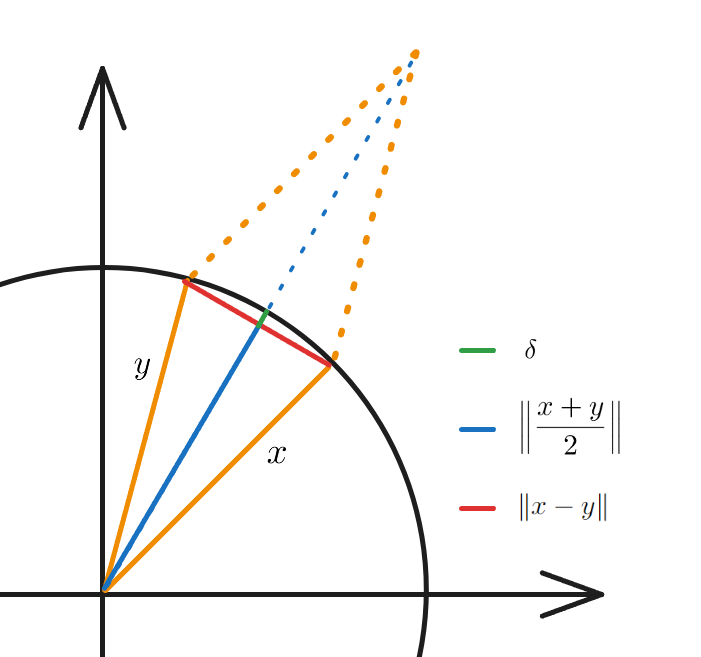
\includegraphics[width=0.4\linewidth]{assets/convex_space_R2.png}
        \caption{$\mathbb R^2$ with $\cnorm_2$ is convex}
        \label{fig:enter-label}
    \end{figure}
    
With the norm 1, $\mathbb R^2$ is not strictly convex.
\begin{figure}[H]
        \centering
        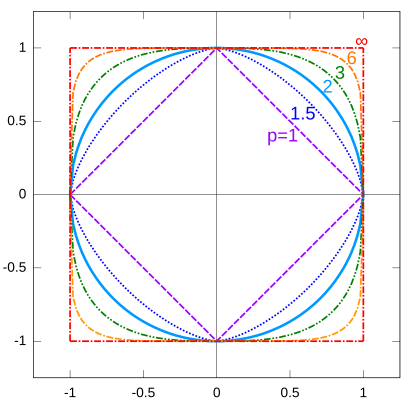
\includegraphics[width=0.4\linewidth]{assets/p-norms_unit_circle_R^2.png}
        \caption{unit circle with p-norms due to Quartl on Wikipedia page “Lp space”}
        \label{fig:enter-label}
    \end{figure}
One can see that in $(\mathbb R^n,\cnorm_p)$ the property is true $\iff 1<p<+\infty$, and fails for $p=1,+\infty$. In fact, from the image above it's easy to see that with 1-norm, the unit ball $B_1$ would be a polytope, and so $\Vert x-y\Vert_1 = \Vert \frac {x+y}2\Vert_1$. The space would be convex, but not strictly convex.

\subsubsection{(thm) Millman-Pettis}
$X$ Banach, uniformly convex $\implies X$ reflexive (i.e. $X^{**}=X$).
\begin{proof}
    omitted. (very difficult)
\end{proof}
\subsubsection{(prop) $L^p(X)$ is uniformly convex}
Take any complete measue space $(X,\mathcal M,\mu)$ and $1<p<+\infty$,\\
then $L^p(X)$ is uniformly convex
\begin{proof}
    Omitted. (based on Clarkson inequalities)
\end{proof}
\subsubsection{(corollary)}
$L^p(X)$ is reflexive for $1<p<+\infty$
\paragraph{Remark}
$L^1(X),\ L^\infty(X)$ 
\subsection{Dual space of $L^p$}
\subsubsection{(thm) Riesz's representation theorem for $(L^p)^*$}
$(X,\mathcal M,\mu)$ complete, $1<p<+\infty$, $\frac 1p+\frac 1{p'}=1$\\
Then $\forall L\in \Big (L^p(X)\Big )^*\quad \exists ! u\in L^{p'}(X)$ s.t. $$Lv =\int_X uv\ \mathrm d \mu, \quad \forall v \in L^p(X)$$
Moreover, $\Vert L\Vert_{(L^p)^*} =\Vert u\Vert _{L^{p'}(X)}$\\
$L_u$ defined as $L_uv=\int_X uv\ \mathrm d\mu$ is an element of $(L^p)^*$ and $\Vert L_u\Vert_{(L^p)^*}=\VErt u\Vert _{L^{p'}}$
Moreover, $T:L^{p'}\xrightarrow[\quad]{}(L^p)^*$ we obtain that $T$ is an isometric isomorphism.
\begin{proof}
    By the properites of isometries and the "example of last time", the only thing left to prove is that $T$ is surjective. This can be done using Hahn-Banach corollaries.
    
\end{proof} 
\subsubsection{(thm) Riesz \#2}
If $p=1$, $(X,\mathcal M,\mu)\quad \sigma$-finite\\
then the $T:L^\infty\to (L^1)'$ is an isomorph isometry.
Finally, $p=+\infty $
$$L^1\hookrightarrow(L^\infty)^*$$
\paragraph{Remark}
The dual of $L^\infty$ is not $L^1$.
\paragraph{Example}
$\forall u\in L^1$, $L_u\in (L^\infty)^*$ but $(L^\infty)^*$ contains elements which do not come from $L^1$.\\
Take $L^\infty([-1,1])$ and consider the space of continuous functions $C([-1,1])$
$$C([-1,1])\subset L^\infty([-1,1])$$
Take $L_0\ : \ C([-1,1])\to \mathbb R$ Just take v from $C([-1,1])$ and evaluate $v(0)$.\\
Check that $L_0$ is linear and $|L_0v|=|v(0)|\leq \Vert v\Vert _\infty$, so that $L_0\in (C([-1,1]))^*$.\\
By Hahn-Banach (with $X=L^\infty, \ Y=C, \ L_0=L_0$) $\implies \exists \tilde L_0$ extension of $L_0$ to $L^\infty$:
$$\begin{cases}
    \tilde L_0\in (L^\infty ([-1,1]))^*\\
    \tilde L_0v=L_0v\quad \forall v\in C([-1,1])\\
    \Vert \tilde L_0\Vert _{(L^\infty)^*}=\Vert L_0\Vert_{(C)^*}\leq 1
\end{cases}$$
\paragraph{Claim} $\nexists u\in L^1([-1,1])$ s.t. $\tilde L_0w=\int_{-1}^1 uw\ \mathrm d\lambda\quad \forall w \in L^\infty$.\\
\begin{proof}
    To show it, by contradiction, assume $\exists u \in L^1$ s.t. $\int_{-1}^1 uw\ \mathrm d \lambda =\tilde L_0 w\quad \forall w \in L^\infty$.\\
Take $$w_n=\begin{cases}
    1-n|x|\quad \text{for }|x|<\frac 1n\\0\quad \quad \text{else}
\end{cases}$$
%insert graph
Show that 
\begin{itemize}
    \item $w_n(0)\to 0$ a.e.
    \item $|w_n(x)|\leq 1$ a.e.
    \item $(w_nu)(x)\to 0$ a.e.
    \item $|w_n(x)u(x)|\leq |u(x)|\in L^1$
\end{itemize}
By dominated convergence,
$$\int_{-1}^1 u w_n\ \mathrm d\lambda \xrightarrow[n\to +\infty]{} 0$$
But the integral is equal to $\tilde L_0 w_n$
$$\tilde L_0 w_n = L_0w_n=w_n(0)=1$$
That is a contradiction
\end{proof}
\paragraph{Resuming}
We have analyzed the properties of $L^p$ spaces: completeness, separability, reflexivity, dual
\[
\begin{array}{|c|c|c|c|c|}
\hline
\textbf{Space} & \textbf{Completeness} & \textbf{Separability} & \textbf{Reflexivity} & \textbf{Dual Space} \\ \hline
L^p, \ 1<p<+\infty & \text{Yes} & \text{Yes} & \text{Yes} & L^{p'}, \ \frac{1}{p}+\frac{1}{p'}=1 \\ \hline
L^1 & \text{Yes} & \text{Yes} & \text{No} & L^\infty \\ \hline
L^\infty & \text{Yes} & \text{No} & \text{No} & \supset L^1 \\ \hline
\end{array}
\]

\subsection{Convergene of sequences}
If we want to solve $Lx=x$, we can iterate $x^{(k+1)}=Lx^{(k)}$\\
$L:\mathbb R^n\to \mathbb R^n,\quad \{x^{(k)}\}$ bounded $\implies x^{(k_j)}\to \bar x$\\
$L$ continuous $\implies \bar x=L\bar x$.\\
If $\dim(X)=+\infty$, boundedness $\centernot\implies$ compactness.\\
To recover compactness, we can either ask more assumptions on the operator (this leads to compact operators) or ask less requirements on the notion of convergence (this leads to the weak convergence approach).
\subsection{Weak Convergence}
\subsubsection{(def) }
Consider $X$ Banach,  $\{ x_n\}_{n\in \mathbb N}\subset X,\quad x\in X$.
We say that $x_n$ weakly converges to $x$,
$$x_n\rightharpoonup x\text{ (weakly) in }X \text{ (for }n\to+\infty)$$
if $\forall L\in X^*$,
$$Lx_n\xrightarrow[\quad]{}Lx\quad(\text{ in }\mathbb R)$$
\paragraph{Remark}
If $x_n\xrightarrow[\quad ]{}x$ strongly, $f:X\to Y$ continuous,
$$\implies f(x_n)\xrightarrow[\quad]{}f(x)$$
Since $L\in X^*\implies L$ continuous,
$$\implies Lx_n\xrightarrow[\quad]{}Lx$$
\textbf{So if $\{x_n\}_n$ converges strongly, then $\{x_n\}_n$ converges weakly}
Actually, in $\mathbb R^n$,
$$\text{strong convergence} \iff \text{weak convergence}$$
In a general space $X \quad x_n\to x \substack{\implies \\ \centernot\impliedby}x_n\rightharpoonup x$
\paragraph{Remark}
$1\leq p<+\infty$
$u_n\rightharpoonup u$ in $L^p(X)$ $\iff$ $L_{u_n}\to L_u\quad \forall L\in (L^p(X))^*$
(with $L\in (L^p(X))^* = L_w\quad ,w\in L^{p'}(X)$)
$$\iff\int_Xwu_n\ \mathrm d\mu\to \int_Xwu\quad \forall w\in L^{p'}(X)$$
(Usually one say "testing the sequence on $w$")
\paragraph{Typical error} Weak convergence in $L^p$ is NOT related to a.e. convergence. But see next prop
\subsubsection{(prop) Weak and a.e. conv. implies strong a.e. conv.}
If $u_n\rightharpoonup u$ and $u_n\to u$ a.e. $\implies u_n=u$ a.e.
\subsubsection{Basic properties}
\begin{enumerate}
    \item \textbf{Prop 1}: If it exists, the weak limit is unique
    \begin{proof}
        $$\{x_n\}_n\subset X \implies \substack{x_n\rightharpoonup y\\ x_n\rightharpoonup z}\text{ weakly in} X$$
        $\implies Ly=Lz\quad \forall L\in X$\\
        $\implies y=z \quad$ by a corollary of Hahn-Banach.
    \end{proof}
    \item \textbf{Prop 2}: If $x_n\rightharpoonup x$ weakly in $X$, then $\{x_n\}_n$ is bounded.
    \begin{proof}
    Use Banach-Steinhaus in $X^*$.\\
    Take $\tau (x_n)\in X^{**}$ ($\tau$ canonical map)
    $\forall L\in X^*$,
    $$\\ _{**}\langle\tau (x_n), L\rangle_*\to \ _{**}\langle \tau (x),L\rangle_*$$
    $$\implies \{_{**}\langle\tau (x_n), L\rangle_*\}_n\subset \mathbb R\text{ converges}\implies \text{ it is bounded}$$
    $$\implies \forall L\in X^*\quad \exists M_L>0 \text{ s.t.} \ |_{**}\langle \tau (x_n),L\rangle_*|<M_L\quad \forall n$$
    $$\implies \exists M \text{ s.t.} \ \Vert \tau (x_n)\Vert_{X^{**}}\leq M$$
    $\Vert \tau (x_n)\Vert_{X^{**}}=\Vert x_n\Vert_X$
    
        
    \end{proof}
    \item \textbf{Prop 3}: $x_n\rightharpoonup x$ weakly in $X$, then 
    $$\Vert x\Vert \leq \liminf_{n\to +\infty} \Vert x_n\Vert$$
    \begin{proof}
        By a corollary of Hahn-Banach, if $x\neq 0$,
        $$\exists L\in X^* \ :\ \begin{cases}
            L\bar x=\Vert \bar x\Vert \\
            \Vert L\Vert_*=1
        \end{cases}$$
        Then $$\Vert \bar x\Vert =L\bar x=\lim_n Lx_n = \liminf_{n} Lx_n\leq \liminf_n \Vert L\Vert_*\cdot \Vert x_n\Vert $$
        (we used $Lx_n\leq |Lx_n|\leq \Vert L\Vert_*\Vert x_n\Vert$)
        we observe that $\Vert L\Vert_*=1$
    \end{proof}
    \paragraph{Remark}
    \begin{figure}[h]
        \centering
        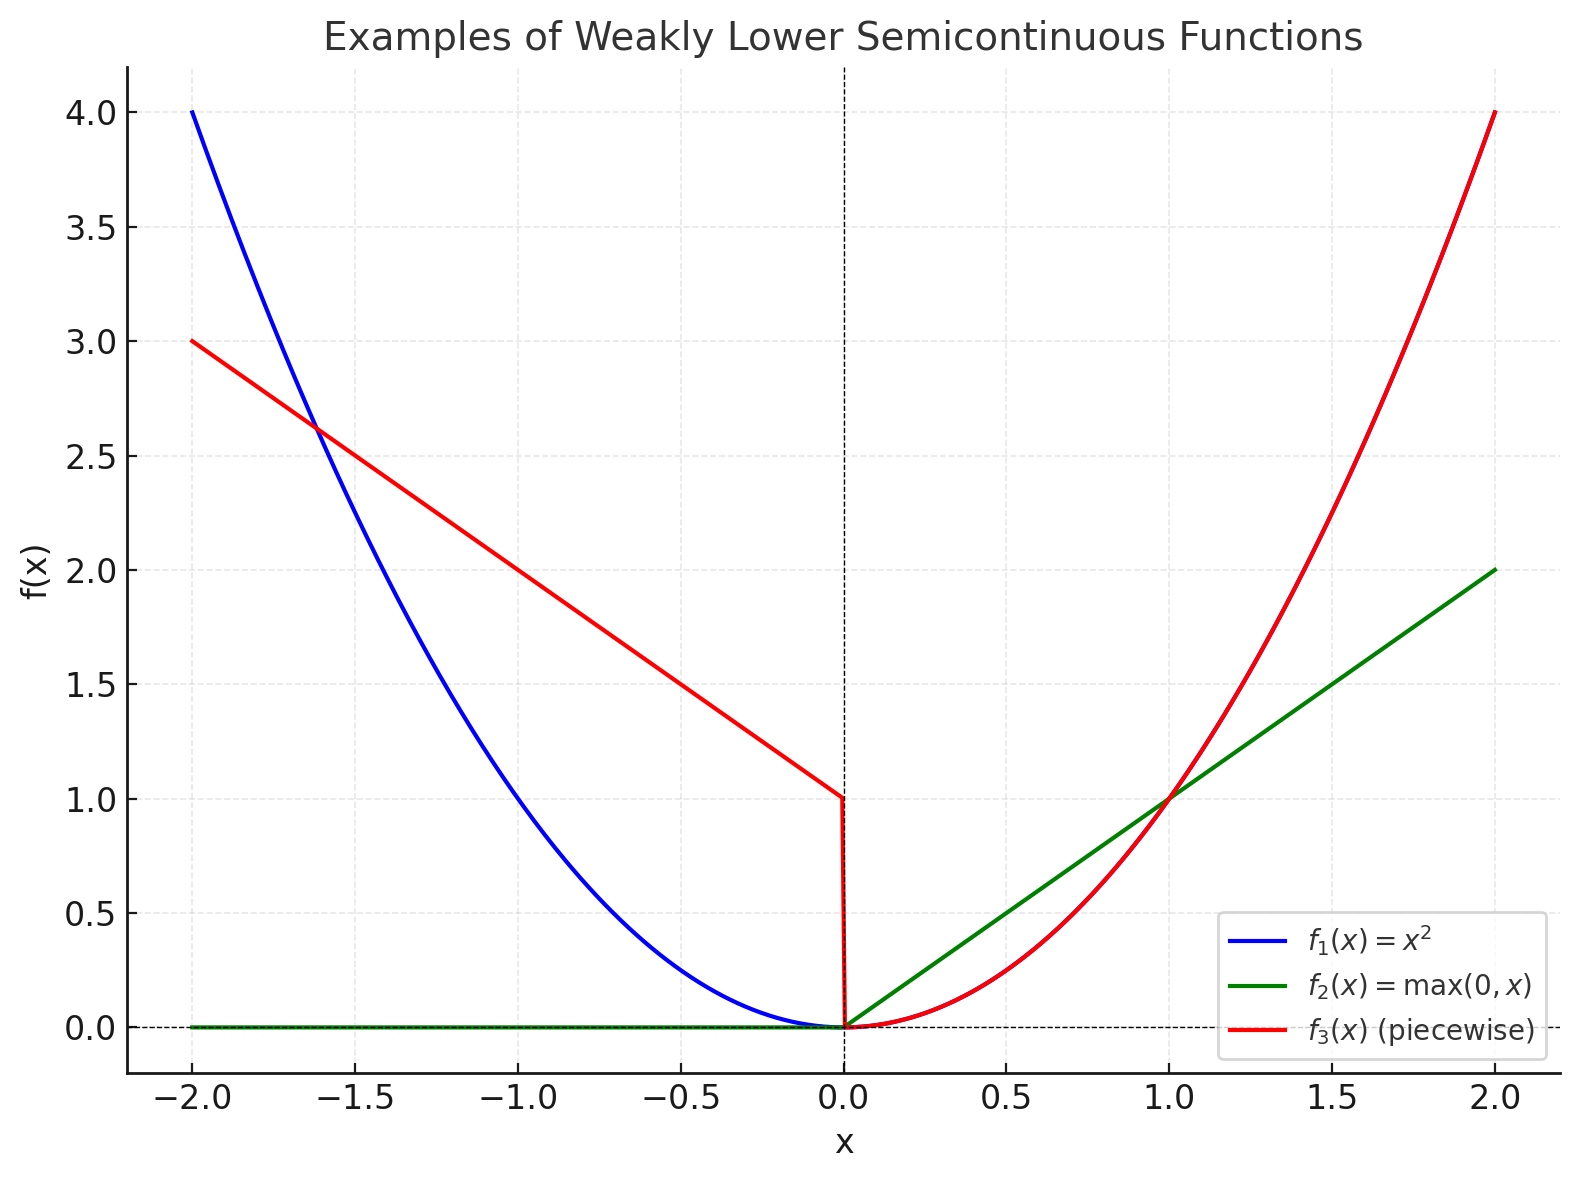
\includegraphics[width=0.5\linewidth]{assets/WEAK.png}
        \caption{Example of weak functions}
        \label{fig:enter-label}
    \end{figure}
    \item \textbf{Prop 4}: $x_n\rightharpoonup x$ weakly in $X$, $L_n\to L$ strongly in $X^*$\\
    Then: 
    $$L_nx_n\to Lx\text{ in }\mathbb R$$
    The same if $x_n\to x$ strongly in  $X$ and $L_n \rightharpoonup L$ weakly in $X^*$\\
    (if both sequences converges weakly, nothing can be inferred).
    \begin{proof}
        Assume $x_n\rightharpoonup x$, $L_n\to L$\\
        $$0\leq|L_nx_n-Lx|=|L_nx_n-Lx_n+Lx_n-Lx|$$
        $$\leq |L_nx_n-Lx_n|+|Lx_n-Lx|$$
        Observe that $|Lx_n-Lx|\to 0$ since $x_n\rightharpoonup x$
        $$\leq \Vert L_n-L\Vert_*\Vert x_n\Vert $$
        But $\Vert L_n-L\Vert_*\to 0$ and $\Vert x_n\Vert$ is bounded by prop 3.\\
        Try to work out the other case by yourself.
    \end{proof}
    \item \textbf{Prop 5}: Take a $X$ Banach space and $V\subset X^*$ dense, $\{x_n\}_n\subset X$ bounded.\\
    Then, if $Lx_n\to Lx\quad \forall L\in V$, then
    $$Lx_n\to Lx\quad \forall L\in X^* \quad (\text{i.e.}\ x_n\rightharpoonup x)$$
    \begin{proof}
        Omitted (similar to the one in prop 4: $V$ dense $\iff$ $\forall L\in X^* \ \exists \{L_n\}_n\subset V$ s.t. $\Vert L_n-L\Vert_*\to 0$)
    \end{proof}
    \paragraph{Example}
    Recall that $1< p<+\infty$, then $u_n\rightharpoonup u$ in $L^p(\Omega)$
    $$\int_{\Omega}u_n v\ \mathrm d\mu\to \int_{\Omega}uv\ \mathrm d\mu \quad \forall v\in L^{p'}(\Omega)$$
    By property 5, it is enough to ask that $\{u_n\}_n\subset L^p(\Omega)$ is bounded and $$\int_\Omega u_uv\ \mathrm d\mu\to \int_\Omega uv\ \mathrm d\mu \quad \forall v \in C_c(\Omega)$$ 
    (or $\forall v\in \text{simple functions}$)
    \item \textbf{Prop 6}: $X,Y$ Banach, $T\in \mathcal L(X,Y)$,
    $$\{x_n\}_n\subset X, \quad x_n\rightharpoonup x \text{ weakly in }X\implies Tx_n\rightharpoonup Tx\text{ weakly in }Y$$
    ($T\in \mathcal L(X,Y)$ is "weakly-weakly continuous")
    
    
\end{enumerate}

%add graph

\subsubsection{(def) Weak$-*$ convergence}
Take $X$ Banach and $X^*$ Banach,
$$\{L_n\}_{n\in \mathbb N}\subset X^*, \ L\in X^*$$
We say that $L_n$ weakly$-*$ converges to $L$
$$L_n\stackrel{\ast}{\rightharpoonup}L$$
if $\forall x\in X$,
$$L_nx\xrightarrow[n\to +\infty]{} Lx$$
\paragraph{Remark}
\begin{itemize}
    \item $L_n\rightharpoonup L$ weakly in $X^*$ if $\phi L_n\to \phi L\quad \forall \phi \in X^{**}$
    \item $L_n\stackrel{\ast}{\rightharpoonup} L$ weakly$-*$ in $X^*$ if $\tau (x)L_n\to \tau (x)L\quad \forall x\in X$
\end{itemize}

\subsection{2/12/2024}
\subsubsection{(rmk)}
In general, weak convergence implies weak-$*$ convergence. But the converse may fail.

\subsubsection{Properties (of weak-$*$ convergence)}
\begin{enumerate}
    \item If $L_n\weakstar L$, then the limit is unique
    \item If $Ln\weakstar L$, then $\{L_n\}_n$ is bounded in $X^*$ nad $\Vert L\Vert_*\leq \liminf_n \Vert L_n\Vert_*$
    \item $$\begin{cases}
        L_n\weakstar L \quad \text{in }X^*\\
        x_n\xrightarrow[\quad]{}x \quad \text{in }X
    \end{cases}\implies L_nx_N\to Lx\quad \text{in }\mathbb R$$
\end{enumerate}
\subsubsection{(rmk)}
The notions of (topological) dual, weak convergence, weak-$*$ convergence, do not need norms, just a topology.
(e.g. "test functions" $\mathcal D(\mathbb R^n)=C_c^\infty(\mathbb R^n)$ and the topological dual of this is $\mathcal D'(\mathbb R^n)$ "distributions" and convergence in $\mathcal D'$ is the weak-$*$ one.
\subsubsection{(rmk)}
we define weak (weak-$*$) convergence, not the weak (weak-$*$) topology. In general, it is not "metrizable" and weakly compact $\centernot\iff$ weakly sequentially compact.
\subsubsection{(thm) Banach-Alaoglu theorems}
\paragraph{Variant 1}
$X$ Banach, reflexive.\\
Then every bounded sequence $\{x_n\}_{n\in \mathbb N}\subset X$ admits a subsequence which weakly converges in $X$.
\paragraph{Variant 2}
$X$ Banach, seqparable.\\
Then every bounded sequence $\{L_n\}_{n\in \mathbb N}\subset X^*$ admits a subsequence $\{L_{n_k}\}_k$ which weakly-$*$ converges in $X^*$
\paragraph{Example ($L^p$, conclusion}
$1<p<+\infty\implies L^p(\Omega)$ is reflexive.
Moreover, we know that $f_n\rightharpoonup f$ weakly in $L^p$
$$\iff \int_\Omega f_ng \to \int_\Omega fg \quad \forall g \in L^{p'}$$
We get: $\forall \ \{u_n\}_{n\in \mathbb N}\subset L^p(\Omega)$, s.t. $\Vert u_n\Vert_p\leq M\quad \forall n\in \mathbb N$,
$$\exists \{u_{n_k}\}_n, \quad \bar u\in L^p\quad s.t.$$
$$\int_\Omega u_{n_k}v\ \mathrm d\lambda \to \int_\Omega \bar uv\ \mathrm d\lambda, \quad \forall v\in L^{p'}$$
\paragraph{Variant 2}
\begin{itemize}
    \item $L^1(\Omega)$ is separable
    \item $L^\infty(\Omega) =(L^1(\Omega))^*$
\end{itemize}
$\forall \{ u_n\}_n\subset L^\infty (\Omega)\quad s.t. \quad \Vert u_n\Vert_{L^\infty} \leq M$
$$\implies \int_\Omega u_{n_k}v \ \mathrm d\lambda \to \int_\Omega \bar u v \ \mathrm d\lambda \quad , \forall v\in L^1(\Omega)$$
(finally, bounded sequences in $L^1$ have no reason to converge)
\subsection{Compact Operators}
$X,Y$ Banach
\paragraph{Recall}
$F$ set is precompact or relatively compact iff $\overline{F}$ is compact.
\subsubsection{(def) }
Take $K:X\to Y$, linear. It is compact if (equivalent conditions):
\begin{itemize}
    \item $\forall E\subset X$ bounded, its image $K(E)\subset Y$ is precompact (i.e. $\overline{K(E)}$ is compact)
    \item
    $\forall \{x_n\}_n\subset X$, bounded, the sequence $\{ Kx_n\}_{n\in \mathbb N}\subset Y$ admits a (strongly) converging subsequence.
\end{itemize}
\subsubsection{(prop)}
$K:X\to Y$ linear, compact.\\
Then $K$ is bounded: $K\in \mathcal L(X,Y)$
\begin{proof}
    $B_1(0)\subset X$ bounded $\implies \overline{K(B_1(0))}$ compact in $Y$\\
    $\implies \overline{K(B_1(0))}$ is bounded.
\\
i.e. $\exists M>0 \quad s.t.\quad \forall x\in X, \Vert x\Vert_X<1, \ \Vert Kx\Vert_Y\leq M$
\end{proof}
\paragraph{Remark}
The above proposition is no longer true for nonlinear compact operators.
\paragraph{Example/exercise (compactness of the integral map)}
$K:C([0,1])\xrightarrow[\quad]{}C([0,1])$
$u\xrightarrow[\quad]{}Ku$
$$(Ku)(x)=\int_0^Xf(s)\ \mathrm ds\quad \forall x\in [0,1]$$
\paragraph{Exercise}
Prove that $K$ is a compact operator. (hint: take $\{u_n\}_n\subset C([0,1])$ bounded).\\Prove that $\{K u_n\}$ has a converging subsequence, using Ascoli-Arzelà).
\subsubsection{(def)}
$T\in \mathcal L(X,Y)$ has finite rank if $\dim R(T)<+\infty$
\paragraph{Examples}
$T\in X^*$, $C^k([a,b])\to \mathbb P^k$ (polynomials of degree k)
\begin{itemize}
    \item Taylor
    \item Langrange interpolation
\end{itemize}
\subsubsection{(prop)}
$$T \text{ finite rank}\substack{\implies\\\centernot \impliedby} T\text{ compact}$$
\begin{proof}
    $A\subset X \implies T(A)\subset R(T) \cong \mathbb R^n$\\
    $\implies \overline{T(A)}\subset R(T)\cong \mathbb R^n$ bounded, closed $\implies $compact
\end{proof}
\subsubsection{(def)}
We denote with $\mathcal K(X,Y)$:
$$\mathcal K(X,Y)=\{ K\in \mathcal L(X,Y) : K\text{ compact}\}$$
\subsubsection{(thm)}
$\mathcal K(X,Y)\subset \mathcal L(X,Y)$ is a closed vector subspace.
\paragraph{Remark}
To check that $T$ is compact, it is enough to find a sequence $\{ T_n\}\subset \mathcal K(X,Y)\ : \ T_n\to T \text{ in}  \ \mathcal L$
\subsubsection{(thm) Compact operators vs weak convergence}
\begin{enumerate}
    \item  $T\in \mathcal K(X,Y)$, then $$\forall \{x_n\}_n\subset X \ s.t. \ x_n\rightharpoonup x \quad \text{weakly in }X$$
    $$\implies Tx_n\to Tx \quad \text{strongly in } Y$$
    \item if $X$ is reflective, from the first point, we have that $T\in \mathcal K(X,Y)$
\end{enumerate}
\begin{proof}
    see exercise classes
\end{proof}
\paragraph{Useless applcations}
$T\in \mathcal K(X,Y)$,
$x^{(0)}\in X$
$$x^{(k)}=Tx^{(k-1)}\dots$$
Assume $\{ x^{(k)}\}$ bounded $\implies x^{(k_j)}\rightharpoonup \bar x$ weakly\\
$$\implies Tx^{(k_j)}\xrightarrow[]{}T\bar x\quad \text{strongly}$$
\subsubsection{(prop)}
$T\in \mathcal K(X,Y)$, $\dim Y=+\infty$\\
$\implies T$ can not be surjective.
\subsubsection{(prop)}
Take either $T\in \mathcal L(X,Y), \ S\in \mathcal K(Y,Z)$ or $T\in \mathcal K(X,Y), \ S\in \mathcal L(Y,Z)$.\\
Then $S\circ T\in \mathcal K(X,Z)$
\begin{proof}
    trivial, because bounded operators map bounded sets into bounded sets and precompact sets into precompact sets.
\end{proof}
